\documentclass[aspectratio=169]{beamer}
\usepackage[utf8]{inputenc}
\usepackage{amsmath, amssymb, amsthm}
\usepackage{tikz}
\usepackage{pgfplots}
\pgfplotsset{compat=1.17}

\usetheme{Madrid}
\usecolortheme{default}

\title{Derivatives: Essential Rules and Properties}
\author{Mathematics Lecture}
\date{}

\begin{document}

\frame{\titlepage}

\begin{frame}
\frametitle{Outline}
\tableofcontents
\end{frame}

\section{Properties of Exponentials and Logarithms}

\begin{frame}
\frametitle{Exponent Properties}

For any real numbers $a, b > 0$ and real numbers $m, n$:

\begin{enumerate}
\item \textbf{Product:} $a^m \cdot a^n = a^{m+n}$
\item \textbf{Quotient:} $\displaystyle\frac{a^m}{a^n} = a^{m-n}$
\item \textbf{Power of power:} $(a^m)^n = a^{mn}$
\item \textbf{Product power:} $(ab)^n = a^n b^n$
\item \textbf{Quotient power:} $\displaystyle\left(\frac{a}{b}\right)^n = \frac{a^n}{b^n}$
\item \textbf{Negative exponent:} $\displaystyle a^{-n} = \frac{1}{a^n}$
\item \textbf{Zero exponent:} $a^0 = 1$ (for $a \neq 0$)
\item \textbf{Fractional:} $a^{1/n} = \sqrt[n]{a}$
\end{enumerate}
\end{frame}

\begin{frame}
\frametitle{Exponent Examples}

\textbf{Example 1:} Simplify $2^3 \cdot 2^5$
$$2^3 \cdot 2^5 = 2^{3+5} = 2^8 = 256$$

\textbf{Example 2:} Simplify $(x^2)^3$
$$(x^2)^3 = x^{2 \cdot 3} = x^6$$

\textbf{Example 3:} Simplify $8^{2/3}$
$$8^{2/3} = (\sqrt[3]{8})^2 = 2^2 = 4$$
\end{frame}

\begin{frame}
\frametitle{Visualizing Exponential Functions}

\begin{center}
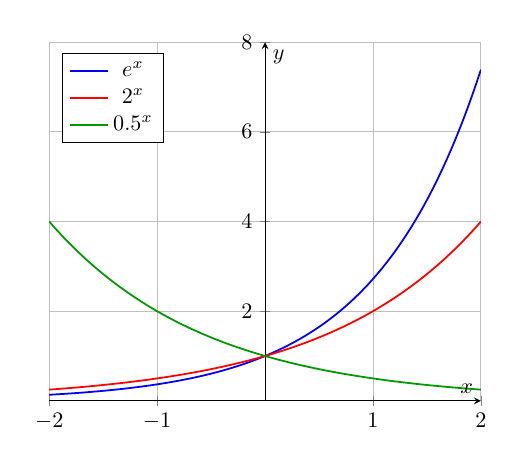
\begin{tikzpicture}[scale=0.8]
\begin{axis}[
    axis lines=middle,
    xlabel={$x$},
    ylabel={$y$},
    domain=-2:2,
    samples=100,
    ymin=0, ymax=8,
    legend pos=north west,
    grid=major
]
\addplot[blue, thick] {exp(x)};
\addlegendentry{$e^x$}
\addplot[red, thick] {2^x};
\addlegendentry{$2^x$}
\addplot[green!60!black, thick] {0.5^x};
\addlegendentry{$0.5^x$}
\end{axis}
\end{tikzpicture}
\end{center}

Notice: $e^x$ and $2^x$ grow, while $0.5^x$ decays as $x$ increases.
\end{frame}

\begin{frame}
\frametitle{Logarithm Properties}

The logarithm $\log_a x$ is the inverse of $a^x$. Natural log: $\ln x = \log_e x$

\vspace{0.3cm}
\textbf{Key Identity:} $a^{\log_a x} = x$ and $\log_a(a^x) = x$

\vspace{0.3cm}
For $a > 0$, $a \neq 1$, and $x, y > 0$:

\begin{enumerate}
\item \textbf{Product:} $\log_a(xy) = \log_a x + \log_a y$
\item \textbf{Quotient:} $\log_a\left(\frac{x}{y}\right) = \log_a x - \log_a y$
\item \textbf{Power:} $\log_a(x^r) = r \log_a x$
\item \textbf{Change of base:} $\log_a x = \frac{\ln x}{\ln a}$
\item \textbf{Special values:} $\log_a 1 = 0$, $\log_a a = 1$
\end{enumerate}
\end{frame}

\begin{frame}
\frametitle{Logarithm Examples}

\textbf{Example 1:} Simplify $\ln(e^{3x})$
$$\ln(e^{3x}) = 3x \ln e = 3x \cdot 1 = 3x$$

\textbf{Example 2:} Expand $\ln\left(\frac{x^2 \sqrt{y}}{z^3}\right)$
\begin{align*}
\ln\left(\frac{x^2 \sqrt{y}}{z^3}\right) &= \ln(x^2) + \ln(\sqrt{y}) - \ln(z^3)\\
&= 2\ln x + \frac{1}{2}\ln y - 3\ln z
\end{align*}

\textbf{Example 3:} Condense $3\ln x - 2\ln y$
$$3\ln x - 2\ln y = \ln(x^3) - \ln(y^2) = \ln\left(\frac{x^3}{y^2}\right)$$
\end{frame}

\begin{frame}
\frametitle{Visualizing Logarithmic Functions}

\begin{center}
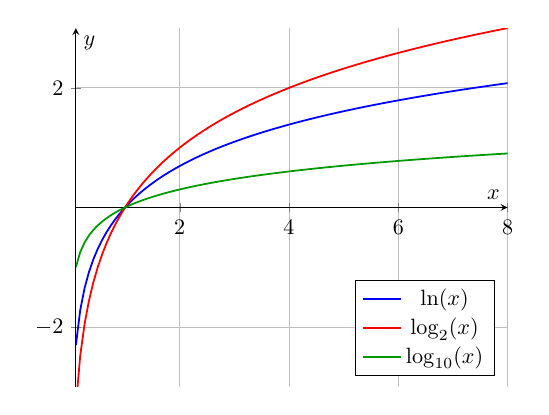
\begin{tikzpicture}[scale=0.8]
\begin{axis}[
    axis lines=middle,
    xlabel={$x$},
    ylabel={$y$},
    domain=0.1:8,
    samples=100,
    ymin=-3, ymax=3,
    legend pos=south east,
    grid=major
]
\addplot[blue, thick] {ln(x)};
\addlegendentry{$\ln(x)$}
\addplot[red, thick] {ln(x)/ln(2)};
\addlegendentry{$\log_2(x)$}
\addplot[green!60!black, thick] {ln(x)/ln(10)};
\addlegendentry{$\log_{10}(x)$}
\end{axis}
\end{tikzpicture}
\end{center}

All logarithms pass through $(1, 0)$ and grow slowly for large $x$.
\end{frame}

\section{Derivative Rules}

\begin{frame}
\frametitle{Sum Rule}

\begin{block}{Sum Rule}
If $f(x)$ and $g(x)$ are differentiable:
$$(f + g)' = f' + g'$$
or equivalently:
$$\frac{d}{dx}[f(x) + g(x)] = \frac{d}{dx}f(x) + \frac{d}{dx}g(x)$$
\end{block}

\vspace{0.5cm}
\textbf{Example:}
$$\frac{d}{dx}(x^3 + 5x^2 - 3x) = 3x^2 + 10x - 3$$

\vspace{0.3cm}
\textbf{Extends to multiple terms:}
$$\frac{d}{dx}[f_1 + f_2 + \cdots + f_n] = f_1' + f_2' + \cdots + f_n'$$
\end{frame}

\begin{frame}
\frametitle{Product Rule}

\begin{block}{Product Rule}
If $f(x)$ and $g(x)$ are differentiable:
$$(f \cdot g)' = f' \cdot g + f \cdot g'$$
\end{block}

\textbf{Mnemonic:} "First times derivative of second, plus second times derivative of first"

\vspace{0.5cm}
\textbf{Example 1:} $\frac{d}{dx}(x^2 \sin x)$
$$\frac{d}{dx}(x^2 \sin x) = 2x \cdot \sin x + x^2 \cdot \cos x$$

\textbf{Example 2:} $\frac{d}{dx}[(3x+1)(x^2-2)]$
\begin{align*}
\frac{d}{dx}[(3x+1)(x^2-2)] &= 3(x^2-2) + (3x+1)(2x)\\
&= 3x^2 - 6 + 6x^2 + 2x = 9x^2 + 2x - 6
\end{align*}
\end{frame}

\begin{frame}
\frametitle{Quotient Rule}

\begin{block}{Quotient Rule}
If $f(x)$ and $g(x)$ are differentiable and $g(x) \neq 0$:
$$\left(\frac{f}{g}\right)' = \frac{f' \cdot g - f \cdot g'}{g^2}$$
\end{block}

\textbf{Mnemonic:} "Low dee-high minus high dee-low, over low-low"

\vspace{0.5cm}
\textbf{Example:} $\frac{d}{dx}\left(\frac{x^2}{x+1}\right)$
\begin{align*}
\frac{d}{dx}\left(\frac{x^2}{x+1}\right) &= \frac{2x(x+1) - x^2(1)}{(x+1)^2}\\
&= \frac{2x^2 + 2x - x^2}{(x+1)^2} = \frac{x^2 + 2x}{(x+1)^2}
\end{align*}
\end{frame}

\begin{frame}
\frametitle{Chain Rule}

\begin{block}{Chain Rule}
If $y = f(g(x))$, then:
$$\frac{dy}{dx} = f'(g(x)) \cdot g'(x)$$

Using Leibniz notation: if $y = f(u)$ and $u = g(x)$:
$$\frac{dy}{dx} = \frac{dy}{du} \cdot \frac{du}{dx}$$
\end{block}

\textbf{Intuition:} Rate of change of $y$ w.r.t. $x$ = (rate of $y$ w.r.t. $u$) $\times$ (rate of $u$ w.r.t. $x$)
\end{frame}

\begin{frame}
\frametitle{Chain Rule Examples}

\textbf{Example 1:} $\frac{d}{dx}(3x+1)^5$

Let $u = 3x+1$, then $y = u^5$
$$\frac{dy}{dx} = 5u^4 \cdot 3 = 15(3x+1)^4$$

\textbf{Example 2:} $\frac{d}{dx}\sin(x^2)$
$$\frac{d}{dx}\sin(x^2) = \cos(x^2) \cdot 2x = 2x\cos(x^2)$$

\textbf{Example 3:} $\frac{d}{dx}e^{x^3+2x}$
$$\frac{d}{dx}e^{x^3+2x} = e^{x^3+2x} \cdot (3x^2+2)$$
\end{frame}

\begin{frame}
\frametitle{Geometric Interpretation of the Derivative}

\begin{center}
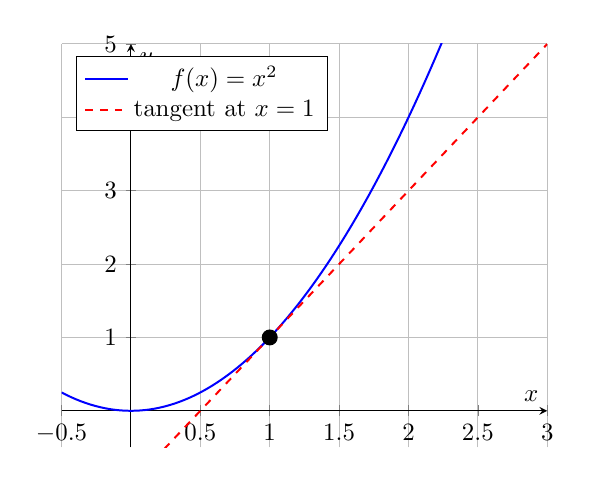
\begin{tikzpicture}[scale=0.9]
\begin{axis}[
    axis lines=middle,
    xlabel={$x$},
    ylabel={$y$},
    domain=-0.5:3,
    samples=100,
    ymin=-0.5, ymax=5,
    grid=major,
    legend pos=north west
]
\addplot[blue, thick] {x^2};
\addlegendentry{$f(x) = x^2$}
\addplot[red, thick, dashed] {2*x - 1};
\addlegendentry{tangent at $x=1$}
\addplot[only marks, mark=*, mark size=3pt] coordinates {(1,1)};
\end{axis}
\end{tikzpicture}
\end{center}

At $x=1$: $f'(1) = 2$, so the tangent line has slope 2.
\end{frame}

\begin{frame}
\frametitle{Combining Rules}

Often we need multiple rules together!

\vspace{0.5cm}
\textbf{Example:} Find $\frac{d}{dx}\left[\frac{(x^2+1)^3}{x}\right]$

Using quotient rule + chain rule:
\begin{align*}
\frac{d}{dx}\left[\frac{(x^2+1)^3}{x}\right] &= \frac{x \cdot 3(x^2+1)^2 \cdot 2x - (x^2+1)^3 \cdot 1}{x^2}\\
&= \frac{6x^2(x^2+1)^2 - (x^2+1)^3}{x^2}\\
&= \frac{(x^2+1)^2[6x^2 - (x^2+1)]}{x^2}\\
&= \frac{(x^2+1)^2(5x^2-1)}{x^2}
\end{align*}
\end{frame}

\section{Common Derivatives}

\begin{frame}
\frametitle{Power Functions}

\begin{align*}
\frac{d}{dx}(c) &= 0 \quad \text{(constant)}\\[0.3cm]
\frac{d}{dx}(x) &= 1\\[0.3cm]
\frac{d}{dx}(x^n) &= nx^{n-1} \quad \text{(power rule)}\\[0.3cm]
\frac{d}{dx}(\sqrt{x}) &= \frac{1}{2\sqrt{x}}\\[0.3cm]
\frac{d}{dx}\left(\frac{1}{x}\right) &= -\frac{1}{x^2}
\end{align*}
\end{frame}

\begin{frame}
\frametitle{Exponential and Logarithmic Functions}

\begin{align*}
\frac{d}{dx}(e^x) &= e^x\\[0.3cm]
\frac{d}{dx}(a^x) &= a^x \ln a\\[0.3cm]
\frac{d}{dx}(\ln x) &= \frac{1}{x}\\[0.3cm]
\frac{d}{dx}(\log_a x) &= \frac{1}{x \ln a}
\end{align*}

\vspace{0.5cm}
\textbf{Note:} The exponential function $e^x$ is special—it's its own derivative!
\end{frame}

\begin{frame}
\frametitle{Visualizing $e^x$ and Its Derivative}

\begin{center}
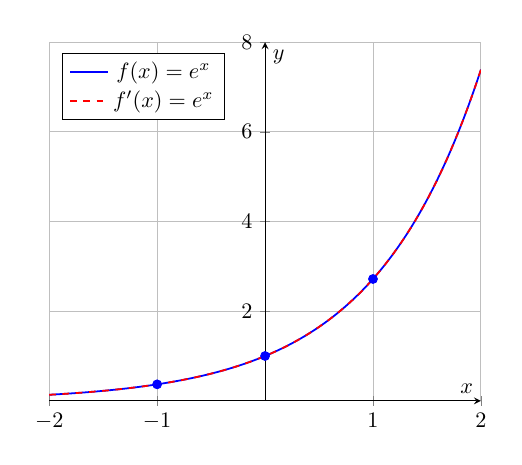
\begin{tikzpicture}[scale=0.8]
\begin{axis}[
    axis lines=middle,
    xlabel={$x$},
    ylabel={$y$},
    domain=-2:2,
    samples=100,
    ymin=0, ymax=8,
    legend pos=north west,
    grid=major
]
\addplot[blue, thick] {exp(x)};
\addlegendentry{$f(x) = e^x$}
\addplot[red, thick, dashed] {exp(x)};
\addlegendentry{$f'(x) = e^x$}
\addplot[only marks, mark=*, mark size=2pt, blue] coordinates {(-1,0.368) (0,1) (1,2.718)};
\end{axis}
\end{tikzpicture}
\end{center}

The function and its derivative are identical! At any point, the slope equals the function value.
\end{frame}

\begin{frame}
\frametitle{Exponential Examples}

\textbf{Example 1:} $\frac{d}{dx}(e^{3x})$
$$\frac{d}{dx}(e^{3x}) = e^{3x} \cdot 3 = 3e^{3x}$$

\textbf{Example 2:} $\frac{d}{dx}(xe^x)$ (product rule)
$$\frac{d}{dx}(xe^x) = 1 \cdot e^x + x \cdot e^x = e^x(1+x)$$

\textbf{Example 3:} $\frac{d}{dx}(2^x)$
$$\frac{d}{dx}(2^x) = 2^x \ln 2$$
\end{frame}

\begin{frame}
\frametitle{Logarithm Examples}

\textbf{Example 1:} $\frac{d}{dx}[\ln(x^2+1)]$
$$\frac{d}{dx}[\ln(x^2+1)] = \frac{1}{x^2+1} \cdot 2x = \frac{2x}{x^2+1}$$

\textbf{Example 2:} $\frac{d}{dx}[x \ln x]$ (product rule)
$$\frac{d}{dx}[x \ln x] = 1 \cdot \ln x + x \cdot \frac{1}{x} = \ln x + 1$$

\textbf{Example 3:} $\frac{d}{dx}(\log_{10} x)$
$$\frac{d}{dx}(\log_{10} x) = \frac{1}{x \ln 10}$$
\end{frame}

\begin{frame}
\frametitle{Trigonometric Functions}

\begin{columns}
\begin{column}{0.5\textwidth}
\begin{align*}
\frac{d}{dx}(\sin x) &= \cos x\\[0.3cm]
\frac{d}{dx}(\cos x) &= -\sin x\\[0.3cm]
\frac{d}{dx}(\tan x) &= \sec^2 x
\end{align*}
\end{column}
\begin{column}{0.5\textwidth}
\begin{align*}
\frac{d}{dx}(\cot x) &= -\csc^2 x\\[0.3cm]
\frac{d}{dx}(\sec x) &= \sec x \tan x\\[0.3cm]
\frac{d}{dx}(\csc x) &= -\csc x \cot x
\end{align*}
\end{column}
\end{columns}
\end{frame}

\begin{frame}
\frametitle{Visualizing $\sin x$ and Its Derivative}

\begin{center}
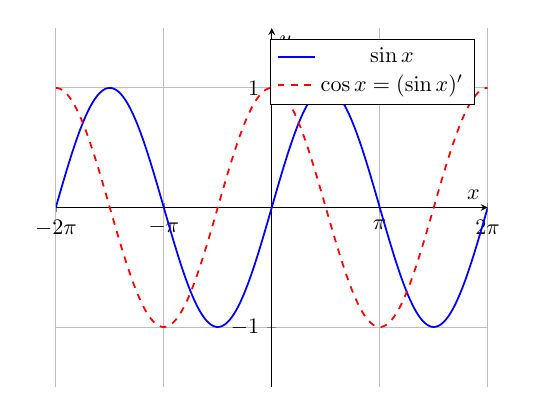
\begin{tikzpicture}[scale=0.8]
\begin{axis}[
    axis lines=middle,
    xlabel={$x$},
    ylabel={$y$},
    domain=-6.28:6.28,
    samples=200,
    ymin=-1.5, ymax=1.5,
    legend pos=north east,
    grid=major,
    xtick={-6.28, -3.14, 0, 3.14, 6.28},
    xticklabels={$-2\pi$, $-\pi$, $0$, $\pi$, $2\pi$}
]
\addplot[blue, thick] {sin(deg(x))};
\addlegendentry{$\sin x$}
\addplot[red, thick, dashed] {cos(deg(x))};
\addlegendentry{$\cos x = (\sin x)'$}
\end{axis}
\end{tikzpicture}
\end{center}

The derivative $\cos x$ represents the slope of $\sin x$ at each point.
\end{frame}

\begin{frame}
\frametitle{Inverse Trigonometric Functions}

\begin{align*}
\frac{d}{dx}(\arcsin x) &= \frac{1}{\sqrt{1-x^2}}\\[0.3cm]
\frac{d}{dx}(\arccos x) &= -\frac{1}{\sqrt{1-x^2}}\\[0.3cm]
\frac{d}{dx}(\arctan x) &= \frac{1}{1+x^2}
\end{align*}
\end{frame}

\section{Higher-Order Derivatives}

\begin{frame}
\frametitle{What are Higher-Order Derivatives?}

The derivative of a derivative!

\vspace{0.5cm}
\textbf{Notation:}
\begin{itemize}
\item \textbf{First derivative:} $f'(x)$ or $\frac{df}{dx}$
\item \textbf{Second derivative:} $f''(x)$ or $\frac{d^2f}{dx^2}$
\item \textbf{Third derivative:} $f'''(x)$ or $\frac{d^3f}{dx^3}$
\item \textbf{$n$-th derivative:} $f^{(n)}(x)$ or $\frac{d^nf}{dx^n}$
\end{itemize}
\end{frame}

\begin{frame}
\frametitle{Physical Interpretation}

If $f(t)$ represents position at time $t$:

\begin{itemize}
\item $f'(t)$ = \textbf{velocity} (rate of change of position)
\item $f''(t)$ = \textbf{acceleration} (rate of change of velocity)
\item $f'''(t)$ = \textbf{jerk} (rate of change of acceleration)
\end{itemize}

\vspace{0.5cm}
Higher derivatives tell us about the \emph{curvature} and behavior of functions!
\end{frame}

\begin{frame}
\frametitle{Visualizing Concavity with Second Derivative}

\begin{center}
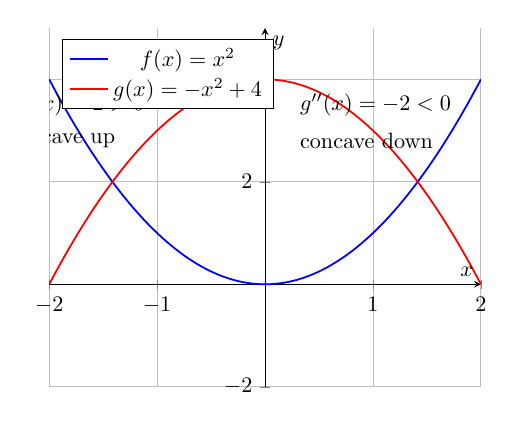
\begin{tikzpicture}[scale=0.8]
\begin{axis}[
    axis lines=middle,
    xlabel={$x$},
    ylabel={$y$},
    domain=-2:2,
    samples=100,
    ymin=-2, ymax=5,
    legend pos=north west,
    grid=major
]
\addplot[blue, thick] {x^2};
\addlegendentry{$f(x) = x^2$}
\node[text width=3cm] at (axis cs: -1.5, 3.5) {$f''(x) = 2 > 0$};
\node[text width=3cm] at (axis cs: -1.5, 2.8) {concave up};
\addplot[red, thick] {-x^2 + 4};
\addlegendentry{$g(x) = -x^2+4$}
\node[text width=3cm] at (axis cs: 1.2, 3.5) {$g''(x) = -2 < 0$};
\node[text width=3cm] at (axis cs: 1.2, 2.8) {concave down};
\end{axis}
\end{tikzpicture}
\end{center}

$f'' > 0$: concave up (U-shaped). $f'' < 0$: concave down ($\cap$-shaped).
\end{frame}

\begin{frame}
\frametitle{Example 1: Polynomial}

Find all derivatives of $f(x) = x^4 - 3x^3 + 2x - 5$

\begin{align*}
f(x) &= x^4 - 3x^3 + 2x - 5\\
f'(x) &= 4x^3 - 9x^2 + 2\\
f''(x) &= 12x^2 - 18x\\
f'''(x) &= 24x - 18\\
f^{(4)}(x) &= 24\\
f^{(5)}(x) &= 0
\end{align*}

All subsequent derivatives are zero!
\end{frame}

\begin{frame}
\frametitle{Example 2: Trigonometric}

Find the first few derivatives of $f(x) = \sin x$

\begin{align*}
f(x) &= \sin x\\
f'(x) &= \cos x\\
f''(x) &= -\sin x\\
f'''(x) &= -\cos x\\
f^{(4)}(x) &= \sin x
\end{align*}

Notice the pattern repeats every 4 derivatives!
\end{frame}

\begin{frame}
\frametitle{Example 3: Exponential}

Find the first few derivatives of $f(x) = e^x$

\begin{align*}
f(x) &= e^x\\
f'(x) &= e^x\\
f''(x) &= e^x\\
f'''(x) &= e^x\\
f^{(n)}(x) &= e^x \quad \text{for all } n
\end{align*}

The exponential function is its own derivative at \emph{every order}!
\end{frame}

\begin{frame}
\frametitle{Practice Problem}

Find $f''(x)$ for $f(x) = x^2 e^x$

\vspace{0.5cm}
\textbf{Solution:}

First derivative (product rule):
$$f'(x) = 2x \cdot e^x + x^2 \cdot e^x = e^x(2x + x^2)$$

Second derivative (product rule again):
\begin{align*}
f''(x) &= e^x(2x + x^2) + e^x(2 + 2x)\\
&= e^x(2x + x^2 + 2 + 2x)\\
&= e^x(x^2 + 4x + 2)
\end{align*}
\end{frame}

\begin{frame}
\frametitle{Summary}

\begin{itemize}
\item \textbf{Exponent/Log Properties:} Essential for simplification
\item \textbf{Sum Rule:} $(f+g)' = f' + g'$
\item \textbf{Product Rule:} $(fg)' = f'g + fg'$
\item \textbf{Quotient Rule:} $\left(\frac{f}{g}\right)' = \frac{f'g - fg'}{g^2}$
\item \textbf{Chain Rule:} $(f \circ g)' = f'(g(x)) \cdot g'(x)$
\item \textbf{Key Derivatives:} $e^x$, $\ln x$, $\sin x$, $\cos x$, $x^n$
\item \textbf{Higher-Order:} Derivatives of derivatives reveal function behavior
\end{itemize}

\vspace{0.5cm}
These tools are fundamental for calculus, optimization, and machine learning!
\end{frame}

\end{document}
